\chapter{Background}
\label{ch:background}

% \lipsum[1]
\todo[inline]{Add a brief introduction to what this chapter will be talking about... etc...}

\section{seL4 Microkernel: A Foundation for Verified Systems}

This section provides an overview of microkernel architecture as a foundation for building high-assurance systems. We begin by discussing the core principles and evolution of microkernel design, followed by an overview of seL4 \citep{klein2009seL4} as a representative third-generation microkernel. Finally, we outline the engineering challenges that arise when building a general-purpose operating systems on top of seL4.

\subsection{What is A Microkernel}

A microkernel is a minimalist approach to operating system kernel design. Unlike a monolithic design, which places all core operating system services -- such as device drivers, file systems, and networking -- within the kernel, a microkernel includes only the most essential components, typically low-level address space management, thread scheduling, and inter-process communication (IPC) \citep{hartig1997ukernel}.

The remaining OS functionality runs in user space as separate, isolated services \citep{hartig1997ukernel}. These components communicate via the aforementioned IPC mechanism. This separation improves modularity, security, and stability, as faults in individual services are less likely to compromise the entire system. However, typical microkernel-based systems often faced performance challenges due to the overhead of IPC and context switching \citep{chen2024hongmeng}.

\begin{figure}[H]
    \centering
    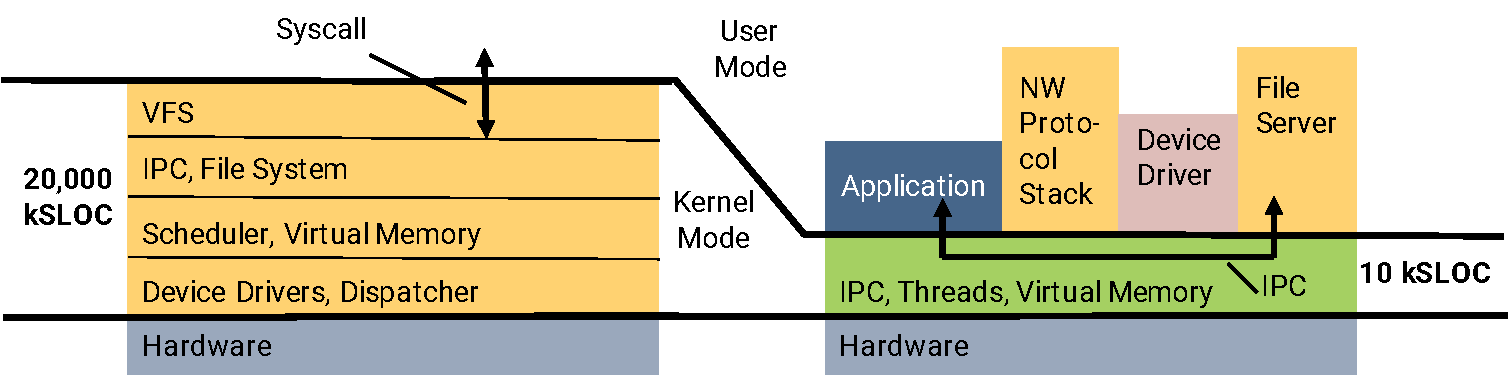
\includegraphics[width=0.65\linewidth]{figs/micro_kernel.pdf}
    \caption{Monolithic (left) vs. Microkernel-based (right) Operating Systems \citep{heiser2025sel4}}
    \label{fig:kernel-comp}
\end{figure}


\subsubsection{Evolution of Microkernel Design}

Microkernel architectures have evolved over time in response to early limitations and shifting system requirements. \autoref{fig:microkernel-gen} illustrates the three major generations of microkernel design \citep{aos2024microkernel}. First-generation microkernels retained much of the functionality typical of monolithic kernels, resulting in many system calls and extremely poor IPC performance. In response, second-generation microkernels embraced minimality as a core principle, stripping unnecessary functionality from the kernel to achieve greater simplicity and significantly improved performance. Third-generation microkernels, such as seL4, further refined this approach by focusing not only on performance but also on formal assurance, including functional correctness and strong isolation guarantees. They achieve this by aggressively minimising the kernel and delegating responsibilities such as memory management to user space.

\begin{figure}[H]
    \centering
    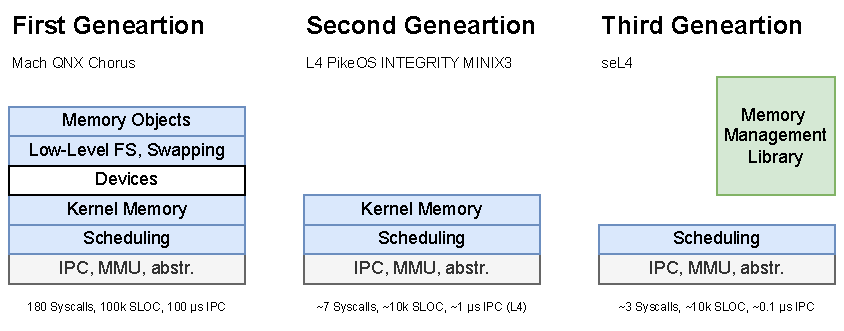
\includegraphics[width=0.65\linewidth]{figs/microkernel-gen.pdf}
    \caption{Generations of Microkernels. Adapted from \citep{aos2024microkernel}}
    \label{fig:microkernel-gen}
\end{figure}

\subsection{The seL4 Microkernel}
seL4 is a third-generation microkernel in the L4 family (\autoref{fig:l4family}), tracing its lineage to Liedtke’s work on high-performance kernels in the mid 1990s \citep{liedtke1995microkernel}. Like its predecessors, seL4 adopts the minimality principle and provides only the essential mechanisms required to securely abstract hardware \citep{heiser2022siot}.

\begin{figure}[H]
    \centering
    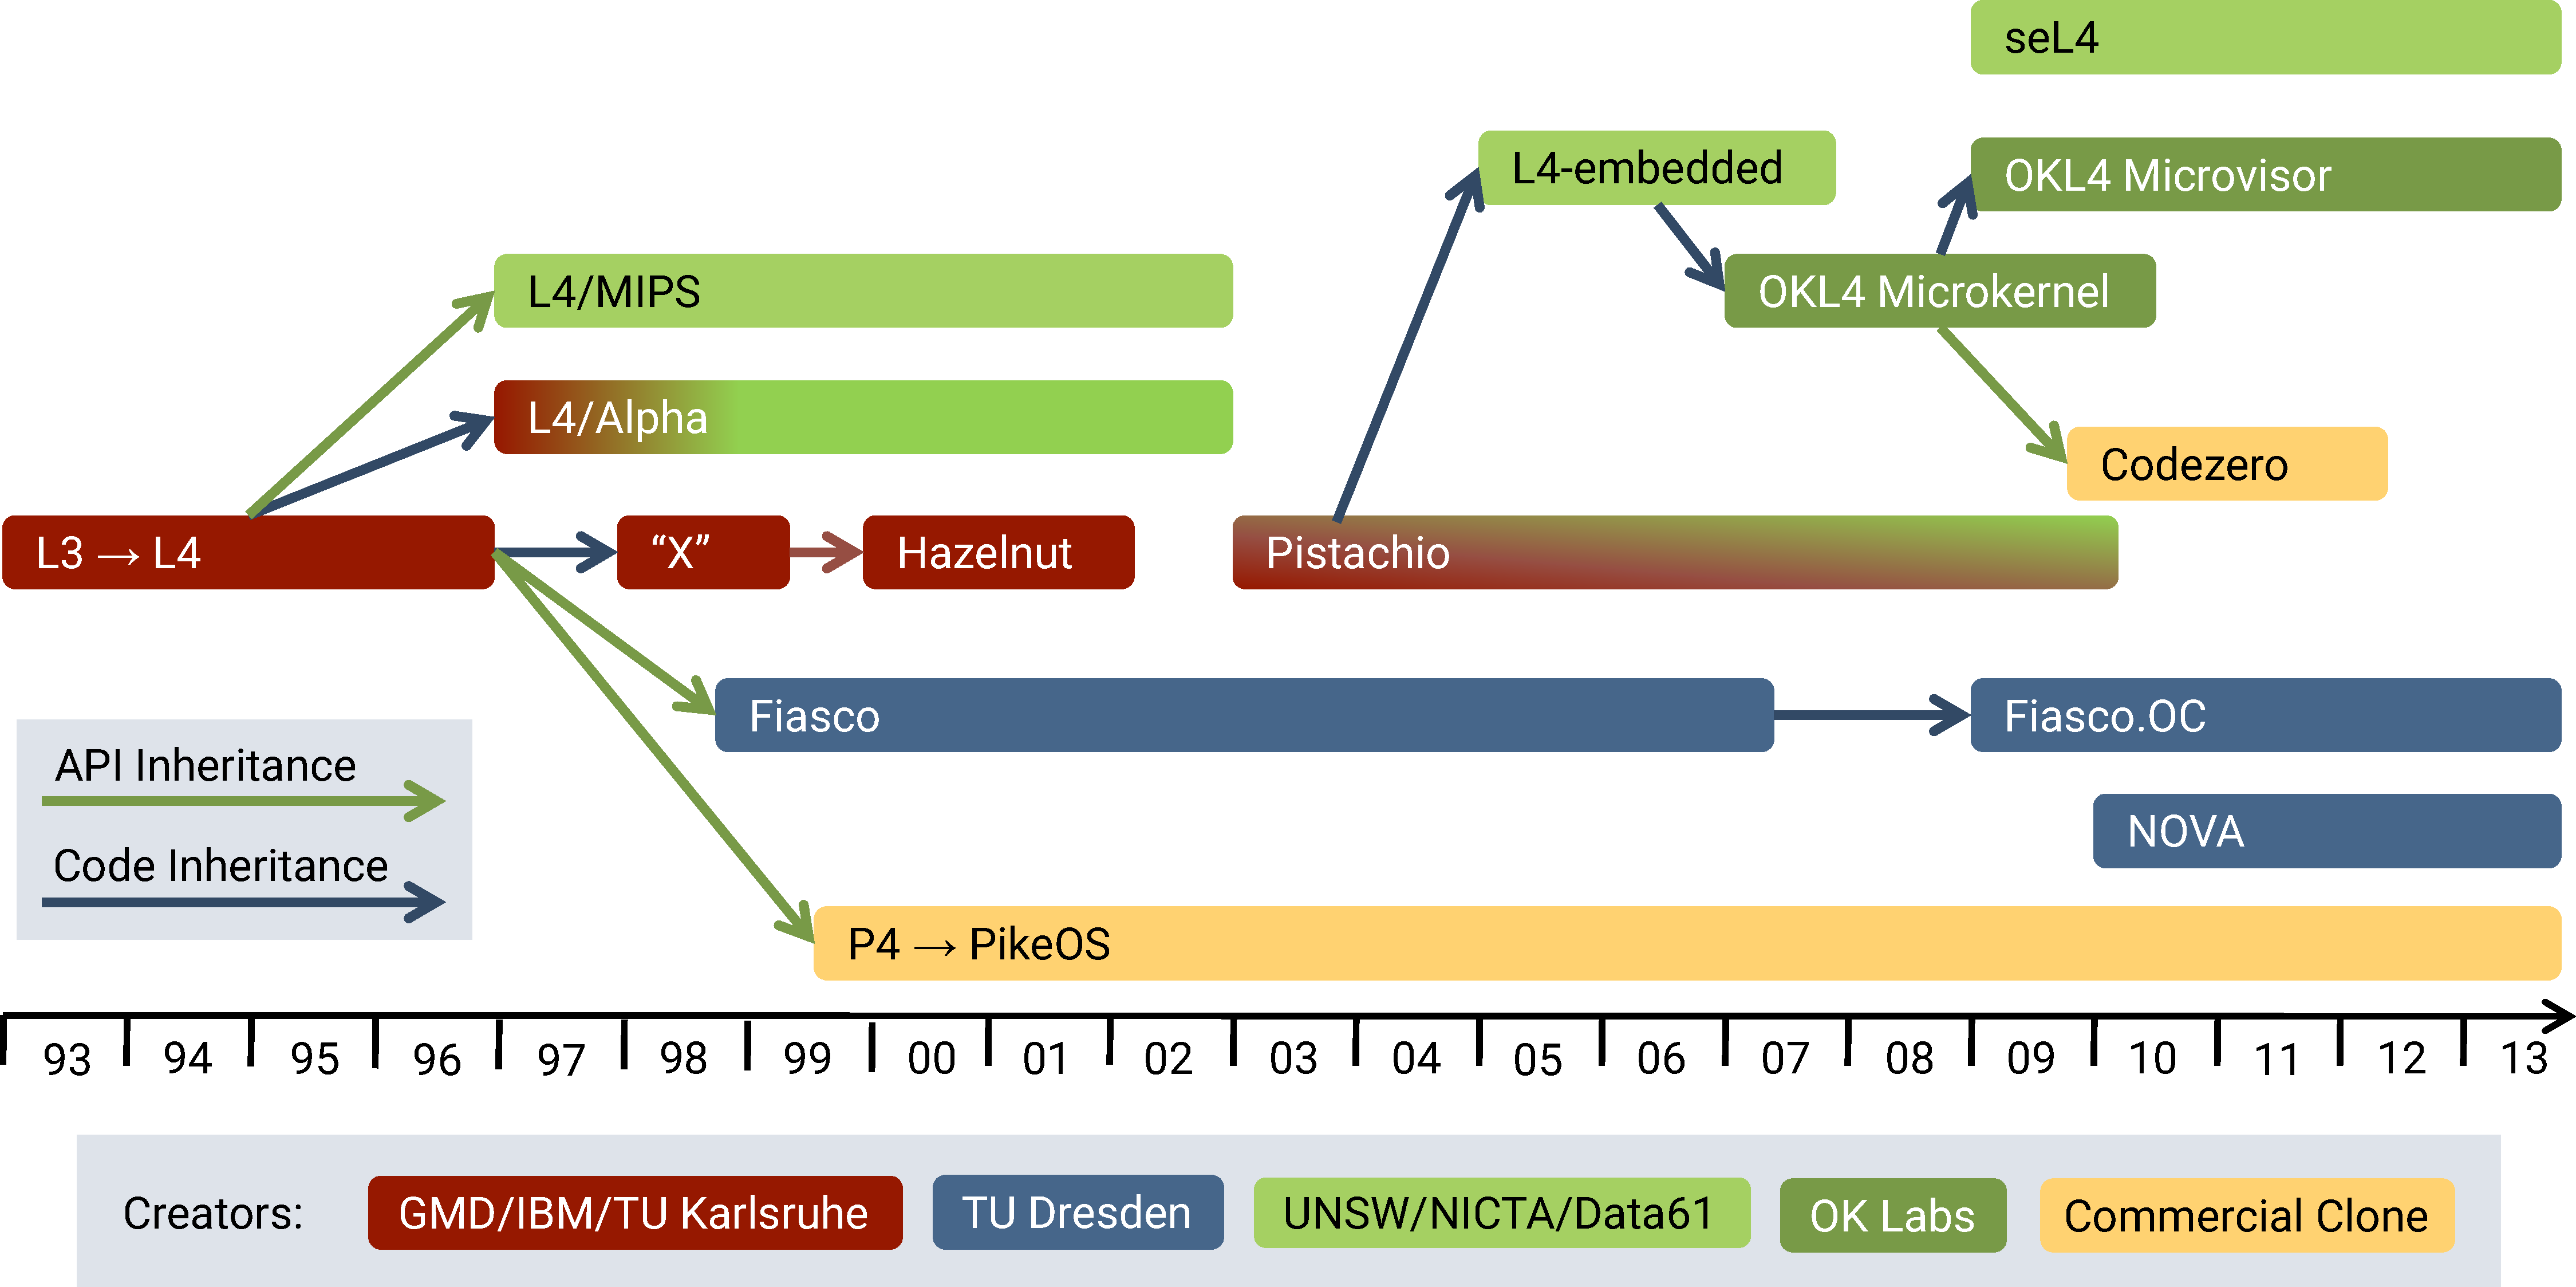
\includegraphics[width=0.65\linewidth]{figs/l4family.pdf}
    \caption{L4 microkernel family tree \citep{heiser2025lionsos}.}
    \label{fig:l4family}
\end{figure}

seL4 combines this minimalist design with strong formal verification: it is the only operating system kernel with machine-checked proofs of functional correctness, integrity enforcement, and confidentiality down to the executable binary \citep{klein2014sel4}. Central to seL4’s security model is its capability-based access control, where capabilities are unforgeable tokens granting specific rights to kernel objects. This model enables fine-grained control and strict spatial isolation between components, ensuring that faults remain contained and cannot compromise the wider system. 

Despite the additional proof infrastructure, empirical studies have established seL4 as the world’s fastest microkernel with performance within 25\% of the limits imposed by hardware it runs on \cite{mi2019skybridge}. These properties make seL4 an attractive foundation for safety- and security-critical systems that require strong isolation, such as autonomous vehicles, medical devices, and industrial control systems. Real-world deployments have demonstrated its potential, including use in autonomous military aircraft \citep{Cofer_GBWPFPKKAHS_18} and commercial electric vehicles \citep{Qu_24:sel4s}. However, such adoptions remain relatively rare and confined to highly specialised domains, reflecting the considerable engineering challenges associated with building practical and general-purpose systems directly on top of seL4’s low-level API.

\subsubsection{Challenges Beyond the Kernel}

While seL4 provides unparalleled assurance and strong isolation properties, its minimal design exposes developers directly to low-level mechanisms that are typically hidden in conventional operating systems. Core responsibilities such as memory management, including page table construction and management of kernel memory regions, are delegated entirely to user space \citep{elkaduwe2008sel4mem}. Although this delegation is critical for enabling provable isolation, it significantly increases the complexity of system construction. Developers must not only reason carefully about the allocation and protection of resources, but must also implement substantial infrastructure before a functional system can even be developed.

As a result, seL4 has often been described as the \emph{``assembly language of operating systems''} \citep{heiser2025lionsos} -- a platform offering fine-grained, powerful primitives, but requiring deep expertise and meticulous engineering to use correctly. For most industrial developers, especially those targeting safety- and security-critical domains, this level of complexity presents a substantial barrier to adoption. Projects that attempt to deploy seL4 at scale without substantial framework support frequently encounter unsustainable engineering overheads, and several early seL4-based initiatives were abandoned after a few years due to these challenges \citep{heiser2025lionsos}. This has motivated several initiatives aiming to address the practical barriers of building systems on seL4, including CAmkES \citep{KUZ2007687} (\autoref{subsec:camkes}), Microkit\citep{microkit:url} (\autoref{subsec:microkit}), and LionsOS \citep{heiser2025lionsos} (\autoref{subsec:lionsos}).

\section{Building Verified Systems on seL4}

Thus far, we have provided a high-level overview of what a microkernel-based operating system looks like, and discussed the challenges involved in building practical systems directly on seL4. In this section, we introduce two key frameworks, CAmkES and Microkit, which aim to reduce the engineering effort required to construct systems on top of seL4. Finally, we present LionsOS, a state-of-the-art operating system built using Microkit, designed to balance security, performance, and practicality.

\subsection{CAmkES}
\label{subsec:camkes}
CAmkES (Component Architecture for microkernel-based Embedded Systems) is a software development and runtime framework designed to simplify the construction of complex multiserver systems on top of the seL4 microkernel. It follows a component-based software engineering approach (see \autoref{fig:camkes-basics}), where a system is modelled as a set of isolated software components with explicitly defined interaction interfaces and connections \citep{KUZ2007687, camkes-docs}.

CAmkES provides a language for describing component interfaces, components themselves, and the overall system architecture. A build tool processes these descriptions and automatically combines developer-provided component code with generated scaffolding and glue code to produce a complete, bootable system image.

\begin{figure}[H]
    \centering
    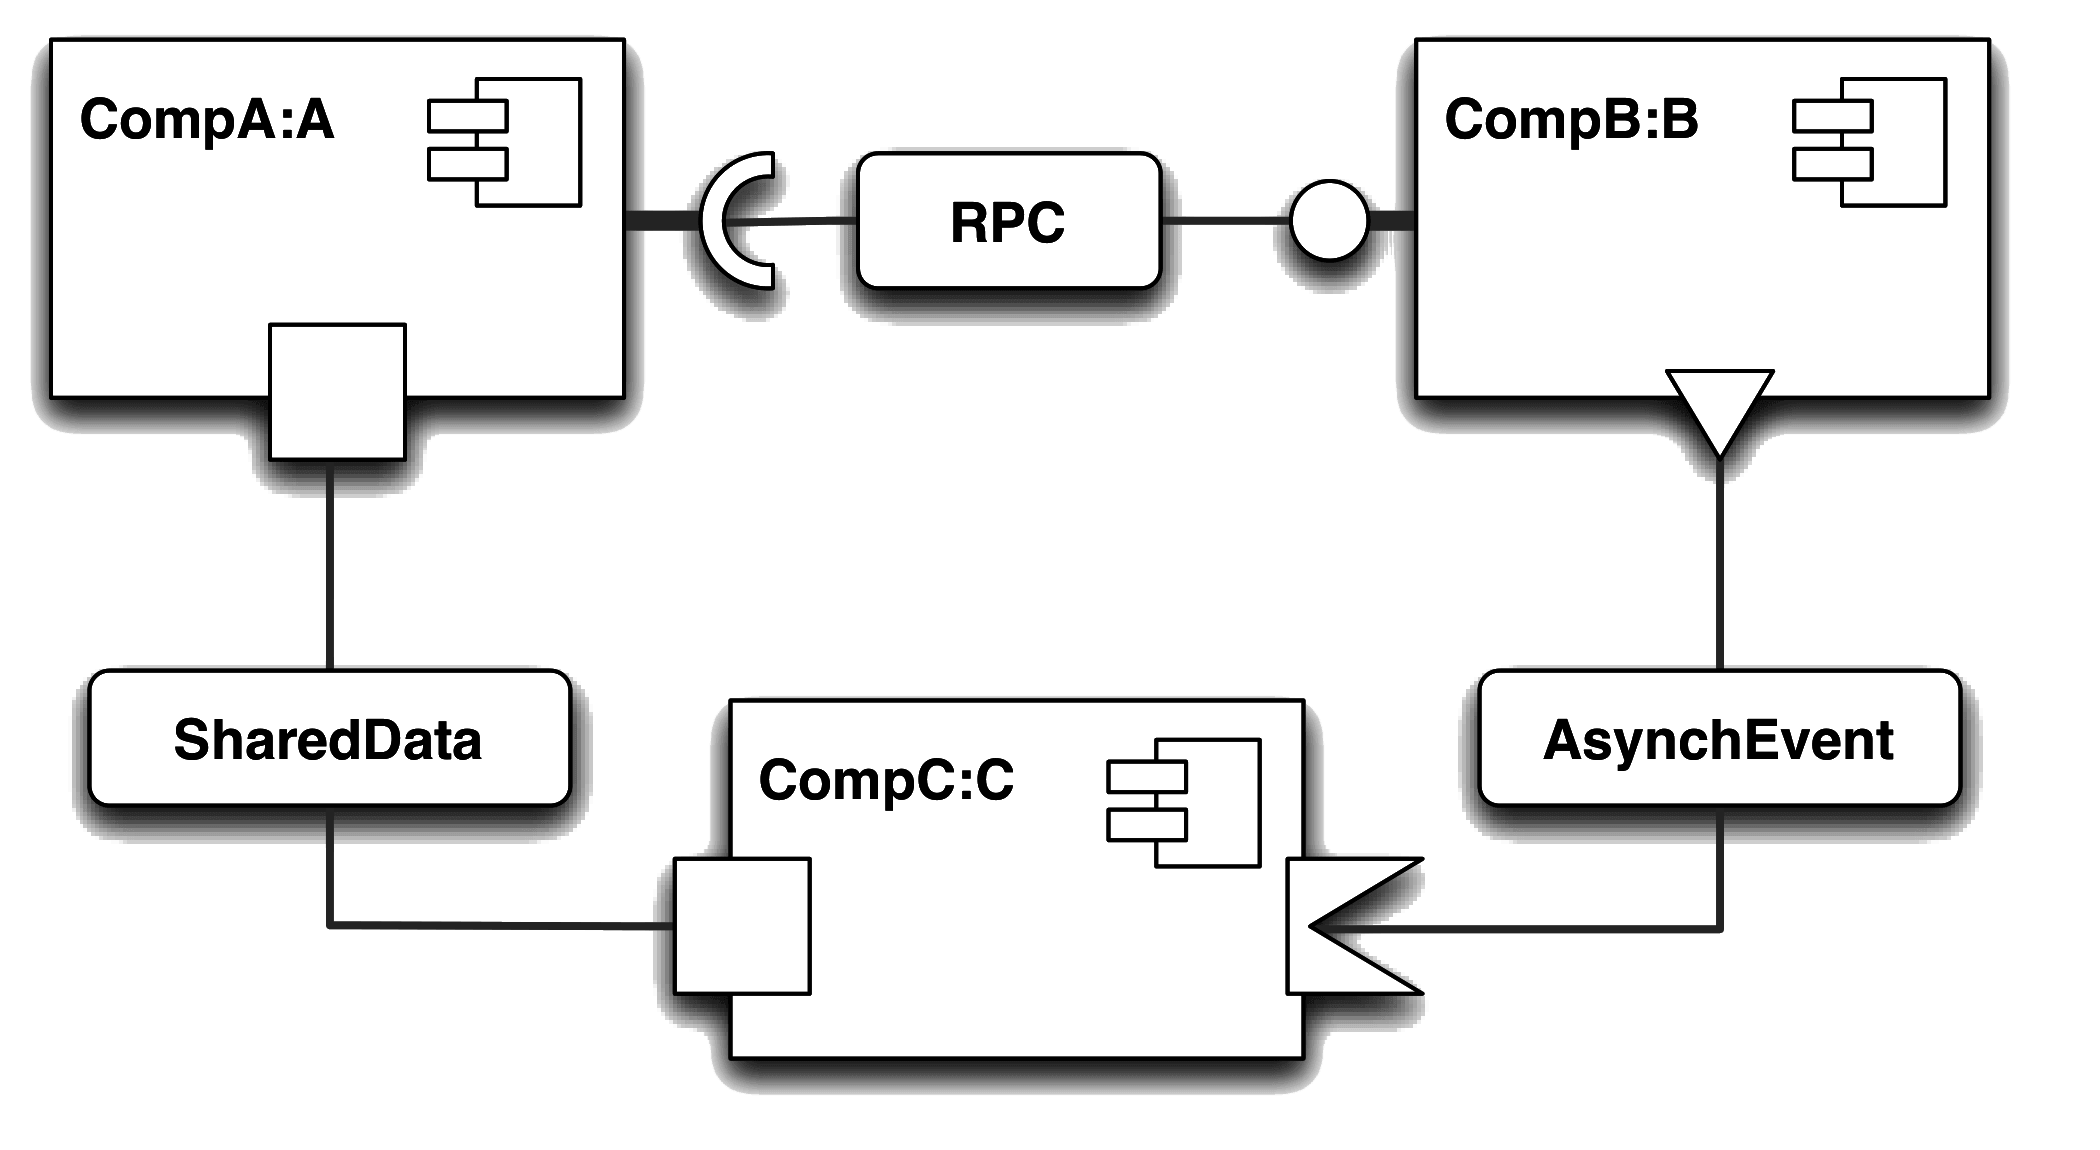
\includegraphics[width=0.65\linewidth]{figs/camkes-basic.png}
    \caption{Basic CAmkES Architecture \citep{camkes-project}}
    \label{fig:camkes-basics}
\end{figure}

However, CAmkES’s abstractions come at a cost. Its component model introduces additional complexity, and its lack of a dedicated software development kit (SDK) results in a cumbersome build process that is tightly coupled to the already complex kernel build system. Furthermore, the generated scaffolding introduces notable runtime overheads \citep{heiser2025sel4}, which can be problematic for performance-sensitive embedded systems. These limitations have motivated the development of more lightweight alternatives, such as Microkit, which aim to simplify system construction while preserving seL4’s strong assurance and performance.


\subsection{The Microkit Framework} 
\label{subsec:microkit}

Microkit was developed as a lightweight framework and software development kit (SDK) for building statically-architecture systems on seL4. It provides a minimal set of simple abstractions that closely mirror seL4’s core mechanisms, enabling developers to construct modular systems with minimal overhead and improved efficiency \citep{microkit-project, microkit:url}.

The central abstraction in Microkit is the Protection Domain (PD), which bundles an address space (VSpace), access rights (CSpace), a thread and scheduling context, and basic synchronisation primitives. A Protection Domain serves as the unit of execution and isolation and is associated with executable code and a scheduling priority. Communication between PDs occurs through user-defined Communication Channels (CCs), which support event notifications and protected procedure calls (PPC). Shared memory communication is also supported through memory objects.

\begin{figure}[H]
    \centering
    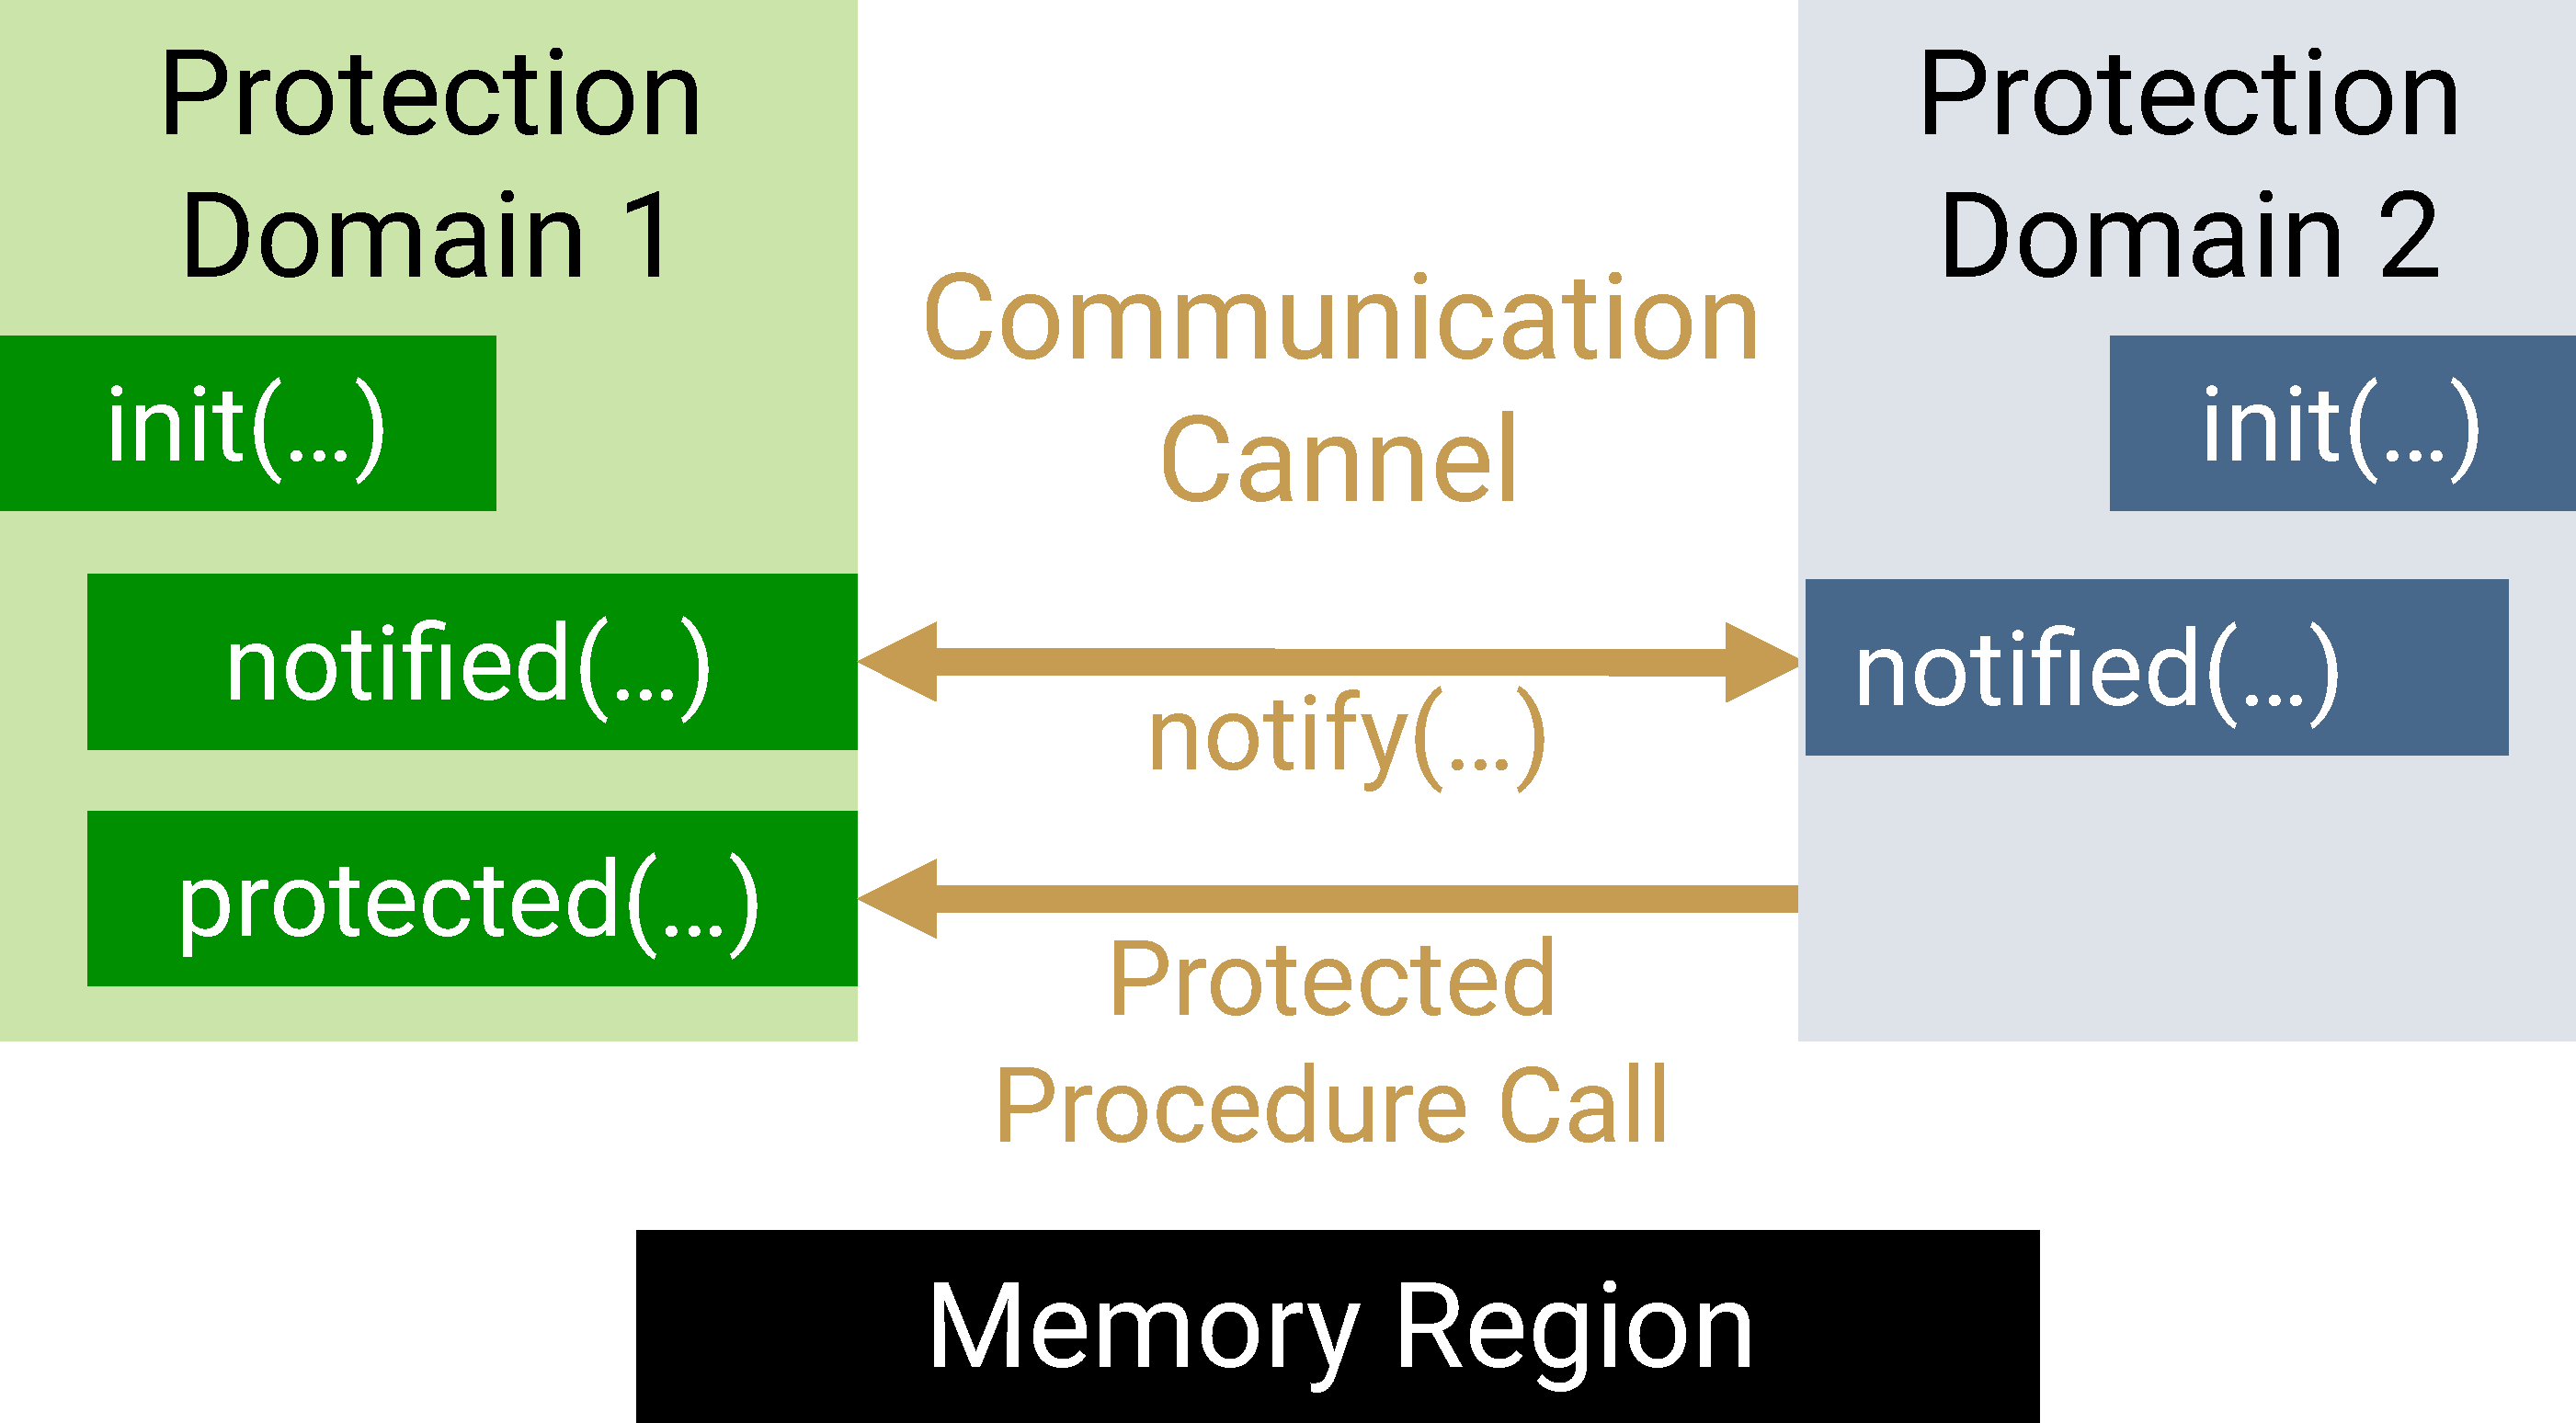
\includegraphics[width=0.65\linewidth]{figs/microkit.pdf}
    \caption{Microkit abstractions \citep{heiser2025sel4}}
    \label{fig:enter-label}
\end{figure}

By intentionally exposing only a small number of abstractions, Microkit encourages developers to design systems that naturally align with seL4’s principles of isolation and minimality. Its communication model further promotes event-driven designs, as Protection Domains are typically structured around asynchronous notifications triggered by Communication Channels. This approach to simplicity not only reduces engineering complexity but also allows formal verification of system behaviour more tractable.

\subsection{LionsOS} 
\label{subsec:lionsos}

LionsOS is a modular operating system designed for safety- and security-critical embedded systems, built on top of the seL4 microkernel and the Microkit framework. It aims to combine the formal assurance and isolation properties of seL4 with a practical and performant system architecture that supports real-world deployment \citep{heiser2025lionsos}.

The design of LionsOS is guided by the principles of strict separation of concerns, least privilege, and \emph{radical simplicity}, following the KISS (``Keep It Simple, Stupid'') principle. Each component is narrowly scoped and operates independently, enabling fine-grained fault isolation and laying the groundwork for scalable formal verification. Rather than attempting to support highly dynamic general-purpose workloads, LionsOS focuses on static system architectures common to embedded and cyberphysical systems, where resource allocation is known ahead of time.

Another key design principle of LionsOS is the use of use-case-specific policies instead of attempting to generalise resource management and scheduling policies across diverse applications. This approach significantly reduces complexity compared to conventional general-purpose OS designs and allows tailored optimisations without sacrificing assurance.

In contrast to earlier attempts at modular, microkernel-based operating systems that suffered severe performance penalties due to high IPC and context-switching costs \citep{chen2024hongmeng}, LionsOS demonstrates that a simple and minimalist approach to OS design can deliver competitive or even superior performance. Empirical evaluation shows that LionsOS exceeds the throughput and latency performance of Linux in network-heavy workloads despite its highly modular architecture \citep{heiser2025lionsos}.


\subsection{The Cost of Verification} 
\label{subsec:verification-cost}

While LionsOS addresses many of the engineering and performance challenges traditionally associated with microkernel-based systems, the issue of formal verification remains a major barrier to achieving a provably secure operating system with a complete end-to-end verification story.

The experience of verifying seL4 demonstrated that functional correctness of real-world operating systems can be formally proven. However, the verification cost was substantial: verifying approximately 8,500 lines of C code required around 12 person-years of work, with an estimated cost of \$350 per line of code \citep{klein2009seL4}. Although such an investment is justified for a operating system kernel, it would be impractical for verifying an entire operating system, which is significantly larger and much more complex.

Recent developments in automated verification have shown that significant reductions in verification effort are possible by leveraging SMT-based techniques instead of traditional interactive theorem proving (ITP). Approaches based on symbolic state-space exploration, guided by heuristics, allow many proof obligations to be discharged automatically without human intervention. These techniques are particularly effective when applied to small, simple modules -- an advantage made possible by LionsOS’s minimalistic and modular system design.

However, even assuming that source-level verification becomes significantly more tractable through automation, a fundamental obstacle remains: ensuring that the compiled binary faithfully implements the verified source code. Without addressing the trustworthiness of the compiler, the overall system cannot achieve true end-to-end assurance. 

In \autoref{sec:compiler-trust}, we will discuss the implications of having the compiler as part of the trusted computing base, namely the challenges posed by unsafe language semantics, compiler optimisations, miscompilations, and the difficulty of ensuring that verified source-level properties are preserved at the binary level. We then examine approaches for addressing these issues through translation validation and verified compilation.

\section{The Compiler Trust Problem}
\label{sec:compiler-trust}
In his 1984 Turing Award Lecture, “Reflections on Trusting Trust,” Ken Thompson revealed a disturbing possibility: even a fully open-source system can have undetectable backdoors if the compiler used to build it is compromised \citep{thompson1984trust}. He described how a maliciously modified compiler could inject a backdoor into an operating system’s \texttt{login} binary and, more insidiously, propagate this backdoor into future compiler binaries -- even if the backdoor no longer appears in any source code. This ``trusting trust'' attack shows that no amount of source-level verification can guarantee system integrity if the compiler itself cannot be trusted.

Even putting aside malicious attacks, compilers are large and complex software systems, and like all such systems, they inevitably contain bugs. Despite decades of engineering effort, miscompilations -- cases where a correct source program is silently translated into an incorrect binary -- remain a recurring problem across all major compiler ecosystems. A large-scale study by \cite{yang2011compilerbugs} found 325 previously unknown bugs across widely used C compilers, including GCC, Clang, and Intel CC, many leading directly to silent miscompilations.

To illustrate the severity of this issue, \autoref{code:gccbug} shows a real-world miscompilation that was introduced in the optimization phase of GCC 9.1\footnote{\url{https://gcc.gnu.org/bugzilla/show_bug.cgi?id=102666}}, where the program would return 0 with no optimisations and 1 with optimisations. It remained unfixed until GCC 12.

\begin{code}
\begin{minted}[linenos, frame=single]{c}
int main(void) {
    for (unsigned a = 0, b = 0; a < 6; a += 1, b += 2)
        if (b < a)
            return 1;
    return 0;
}
\end{minted}
\caption{Example of a miscompilation bug in GCC (Bug \href{https://gcc.gnu.org/bugzilla/show_bug.cgi?id=102666}{\#102666})}
\label{code:gccbug}
\end{code}


For a provably secure system like \textbf{LionsOS}, this problem is not merely theoretical. A single miscompilation, whether due to a malicious injection, a compiler bug, or an unsound optimisation, can undermine the entire verification effort. Since proofs are typically constructed at the source level, the correctness of the resulting binary hinges entirely on the correctness of the compilation process itself. As such, we require techniques that remove the compiler from the TCB and therefore eliminate the need to trust it.

\subsection{Approaches to Removing the Compiler from the TCB}
\subsubsection{Translation Validation}
In seL4's verification story, the compiler was removed from the TCB via a method known as translation validation, where for each individual compilation, the resulting binary is formally shown to refine the verified C source program \citep{sewell2013TV}.

As shown in \autoref{fig:sel4-tv}, the binary is lifted into a control-flow graph representation through a verified disassembler within HOL4, based on a formal ISA model (such as ARM or RISC-V). The C program, already formalised in Isabelle/HOL, is translated into the same graph language through semantics-preserving transformations. To account for compiler optimisations, additional rewrite rules are applied at the graph level within the theorem prover.

The equivalence between the two programs is then checked by splitting them into small chunks and discharging semantic preservation queries to SMT solvers. In theory, establishing full program equivalence is undecidable, as it reduces to the halting problem. In practice, however, the compiler's transformations are sufficiently regular to make the problem tractable for real-world code. Even so, the process remains fragile: minor changes to the source code can alter the structure of these SMT chunks and cause proof attempts to fail. In addition, the toolchain used in the seL4's approach places practical limitations on the complexity of the source code.


\begin{figure}[H]
    \centering
    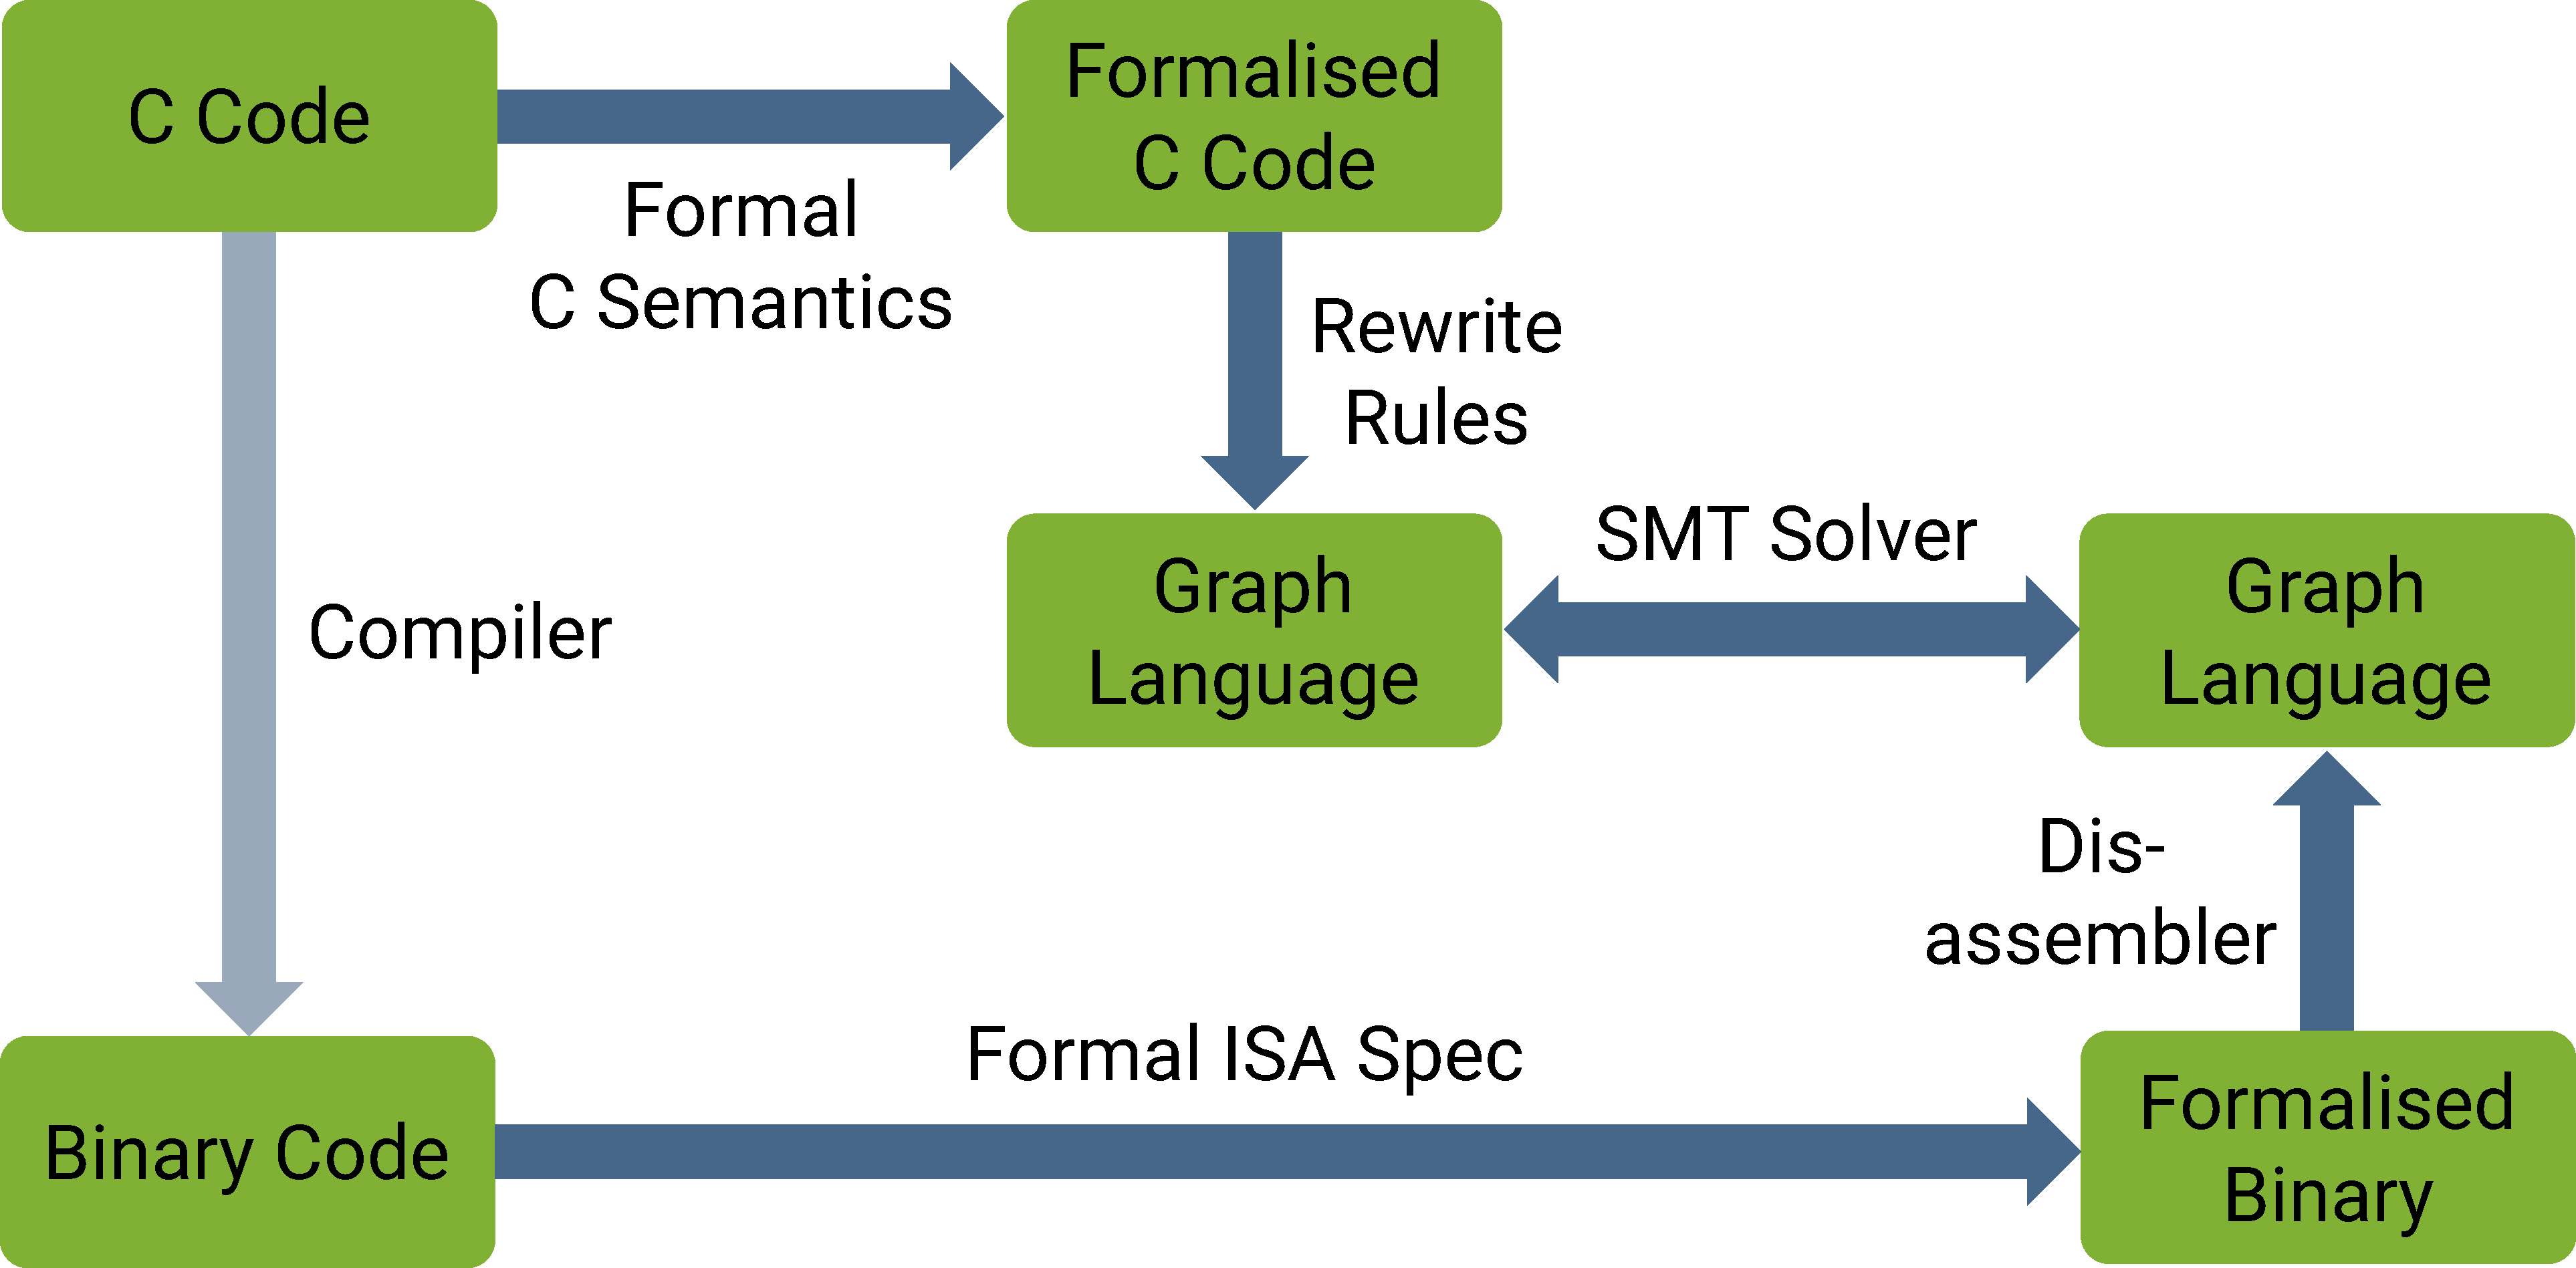
\includegraphics[width=0.65\linewidth]{figs/translation-validation.pdf}
    \caption{Translation validation proof chain \citep{heiser2025sel4}.}
    \label{fig:sel4-tv}
\end{figure}


\subsubsection{Verified Compilers}
A much better alternative to translation validation is the use of a \emph{verified compiler}, where it is guaranteed by construction that the generated binary preserves the semantics of the source program. Rather than verifying each individual compilation after the fact, the correctness of every compilation is a direct consequence of the compiler’s proof.

Although compilers are large and intricate pieces of software, the property they must establish is surprisingly simple: the produced binary must refine the semantics of the input program. Formally, this can often be phrased as a simulation or refinement relation between the source and target languages, typically proved inductively on the structure of the compilation steps. In summary, every transformation applied by the compiler must be proven to preserve or refine the program's observable behaviour. Once this invariant is established for all stages, the compiler can be trusted for all programs within its specification \citep{leroy2009compcert}. This approach eliminates the fragility associated with translation validation and removes the compiler from the TCB entirely.

We will be providing more details on three production-grade verified compilers -- CompCert, Pancake, and CakeML -- in the Related Works section.

